\documentclass{report}
\usepackage[french]{babel}
\usepackage{graphicx}
\usepackage[utf8]{inputenc}
\usepackage{float}
\usepackage{array}
\usepackage{tabularx}
\usepackage[T1]{fontenc}
\usepackage{xcolor}
\usepackage{multirow}


\def\code#1{\texttt{#1}} % pour écrire du code (police monospace)
\def\comment#1{\color{gray} #1 \color{black}}

\begin{document}
\renewcommand{\labelitemi}{$\bullet$}
\renewcommand{\labelitemii}{$\circ$}
\thispagestyle{empty}

\begin{center}
	\vspace*{1cm}
	\huge  \bf Rapport du TP1: Paralèlliser l'algorithme du Crible d'Ératosthène\\
	\vspace{1cm}
	\LARGE Equipe numéro 2\\
	\vspace{1.5cm}
	\normalsize
	\textit{Houssem Sebouai}\\
	111 134 915\\
	houssem.sebouai.1@ulaval.ca\\

  \vspace{1cm}
	\normalsize
	\textit{Thierry St-Gelais}\\
111 169 338\\
thierry.st-gelais.1@ulaval.ca\\

	\vspace{2cm}
	Dans le cadre des travaux pratiques du cours\\
	\LARGE GLO-7014\\
	\large Programmation parallèle et distribuée\\
	Professeur: Marc Parizeau

	\vfill
	
\includegraphics[width=5cm]{Images/logo.jpg}
	\\
	Hiver 2017
\end{center}

\newpage

\tableofcontents
\listoffigures
\listoftables
\newpage
\chapter{Introduction}

	Le but de ce travail était réaliser une algorithme {\it multithread} (multifilaire)
	ayant pour but de trouver les nombre premiers inférieurs à un seuil fixé.
	Nous devions nous inspirer de l'algorithme du Crible d'Ératosthène.

\newpage
\chapter{Description de la méthode}

	\section{Explication de l'algorithme}

		L'algorithme du Crible d'Ératosthène consiste à parcourir un tableau
		en ordre croissant, tout en éliminant successivement les multiples des
		nombres rencontrés du tableau, ou à les {\it flagger} (marquer) comme
		étant des nombres composés et donc, non-premiers.
	\bigskip
	\section{Parralélisation de l'algorithme}

		Dans le cas présent, l'algorithme expliqué ci-haut est parralélisé de
		manière à ce que chaque fil d'exécution prenne en charge un nombre.
		Par exemple, si un premier fil s'occupe de tous les multiples de 2,
		alors le fil suivant marquera tous les multiples de 3, et cetera.

		\bigskip
		\noindent ex.:

		\noindent
		\code{
			\comment{
			1 étant un nombre premier par défaut, il est possible de \\l'ignorer
			dans l'élaboration du code suivant
			} \\
			\\
			lN: entier, \comment{un entier correspondant à la limite de recherche
			pour \\les nombres premiers}\\
			lT: entier, \comment{un entier correspondant au nombre de fils
			d'exécution \\demandés} \\
			\\
			gCand: entier, \comment{Entier qui permet de déterminer les prochains
			\\nombres à marquer} \\
			\\
			N[lN] = [0,0,0, $\ldots$ ,0]: char, \comment{Un tableau de {\it flags}} \\
			\\
			T[lT] = [null, null, $\ldots$ , null]: ptr, \comment{Tableau contenant
			des \\pointeurs vers les différents fils d'exécution} \\
			\\
			Pour (i=2..lT) \\
			\hspace*{16pt} T[i] = créer\_Fil(exec\_Crible(gCand))
		}

		\bigskip
		Ici, les fonctions \code{creer\_Fil()} et \code{exec\_Crible()}
		font exactement ce qu'elles prétendent: la première crée un nouveau fil
		d'exécution qui prendra en charge la fonction passée en paramètre.

		\smallskip
		La seconde, elle, marque dans le tableau les multiples du nombre qui
		lui est passé en paramètre.

\chapter{Expérimenations et résultats}
\section{Protocole d'éxpérimentation}
Nous avons défini dans un script bash le protocole d'éxpériementation suivant:
\begin{itemize}
	\item Nous avons choisi de tester la version séquentiel et parrallèle de l'algorithme du Crible d'Ératosthène
	avec une limite supérieure de $10^{9}$ et ce ci afin d'avoir des temps d'éxécution calculables
	en secondes.\\
	Ces temps d'éxcution nous ont permi de faire une comparaison entre les deux versions de l'algorithme.
	\item Nous avons dévisié cette limite supèrieur en 5 sègements de limite avec une valeur décroissante pour chaque itération.
	C'est à dire, indépendament de la version de l'algoritmhe nous avons fais des tests selon les limites suivantes:
	\begin{itemize}
		\item $10^{9}$
		\item $10^{9}/2=500\times10^{6}$
		\item $10^{9}/3=333\times10^{6}$
		\item $10^{9}/4=250\times10^{6}$
		\item $10^{9}/5=200\times10^{6}$
	\end{itemize}
	\item Nous avons observé par la suite les résultats obtenus en terme de temps d'éxécution.
	\item Nous avons compilé c'est résultat dans des tableaux comapratifs et dans des graphes.
\end{itemize}
\section{Résultats:}
Nous vous présentons dans une première phase les résultats sous la forme de tableaux
comparatifs:
\begin{itemize}
	\item Pour 1'000'000'000 nombres:\\
	\begin{table}[H]
			\center
			\begin{tabular}{|c|c|c|c|}
				\hline
				N\_Thread	&	Time	& SpeedUp	& Efficacité \\
				\hline
				1	&	16,777986	& 1	&	1	\\
				\hline
				2	&	8,115799	& 2,067323994	&	1,033661997	\\
				\hline
				3	&	6,015212	& 2,789259298		&	0,929753099	\\
				\hline
				4	&	4,765035	& 3,521062490	&	0,880265622	\\
				\hline
				5	&	4,505112	& 3,724210630	&	0,744842126	\\
				\hline
				6	&	4,596752	& 3,649965454	&	0,608327576	\\
				\hline
			\end{tabular}
		\caption{Tableau compatratif des résultats 1}
	\end{table}
	\item 500'000'000 nombres:\\
	\begin{table}[H]
			\center
			\begin{tabular}{|c|c|c|c|}
				\hline
				N\_Thread	&	Time	& SpeedUp	& Efficacité \\
				\hline
				1	&	7,625479	& 1	&	1	\\
				\hline
				2	&	3,524735	& 2,163419094		&	1,081709547	\\
				\hline
				3	&	2,877975	& 2,649598763		&	0,883199588	\\
				\hline
				4	&	2,199456	& 3,466984109	&	0,866746027	\\
				\hline
				5	&	2,465800	& 3,092496958	&	0,618499392	\\
				\hline
				6	&	2,432473	& 3,134866862	&	0,52247781	\\
				\hline
			\end{tabular}
		\caption{Tableau compatratif des résultats 2}
	\end{table}
	\item Pour 333'333'333 nombres:\\
	\begin{table}[H]
			\center
			\begin{tabular}{|c|c|c|c|}
				\hline
				N\_Thread	&	Time	& SpeedUp	& Efficacité \\
				\hline
				1	&	5,022416	& 1	&	1	\\
				\hline
				2	&	2,295022	& 2,188395580	&	1,09419779	\\
				\hline
				3	&	1,723167	& 2,914642632		&	0,971547544	\\
				\hline
				4	&	1,408028	& 3,566985884	&	0,891746471	\\
				\hline
				5	&	1,609171	& 3,121120130	&	0,624224026	\\
				\hline
				6	&	1,603027	& 3,133082599		&	0,522180433\\
				\hline
			\end{tabular}
		\caption{Tableau compatratif des résultats 3}
	\end{table}
	\item 250'000'000 nombres:\\
	\begin{table}[H]
			\center
			\begin{tabular}{|c|c|c|c|}
				\hline
				N\_Thread	&	Time	& SpeedUp	& Efficacité \\
				\hline
				1	&	3,752694	& 1	&	1	\\
				\hline
				2	&	1,717787	& 2,184609617	&	1,092304808	\\
				\hline
				3	&	1,376726	& 2,725810365		&	0,908603455	\\
				\hline
				4	&	1,275599	& 2,941907292	&	0,735476823	\\
				\hline
				5	&	1,079926	& 3,474954765	&	0,694990953	\\
				\hline
				6	&	1,170251	& 3,206742827	&	0,534457138	\\
				\hline
			\end{tabular}
		\caption{Tableau compatratif des résultats 4}
	\end{table}
	\item Pour 1'000'000'000 nombres:\\
	\begin{table}[H]
			\center
			\begin{tabular}{|c|c|c|c|}
				\hline
				N\_Thread	&	Time	& SpeedUp	& Efficacité \\
				\hline
				1	&	2,986057	& 1	&	1	\\
				\hline
				2	&	1,367230	& 2,184019514	&	1,092009757	\\
				\hline
				3	&	1,079777	& 2,765438604		&	0,921812868	\\
				\hline
				4	&	0,843836	& 3,538669836	&	0,884667459	\\
				\hline
				5	&	0,849093	& 3,516760826		&	0,703352165\\
				\hline
				6	&	0,929155	& 3,213733984	&	0,535622331\\
				\hline
			\end{tabular}
		\caption{Tableau compatratif des résultats 5}
	\end{table}
\end{itemize}
Par la suite nous vous présentons une compilation des résultats précédents dans les réprésentations graphiques
suivantes:
\begin{center}
	\begin{figure}[H]
		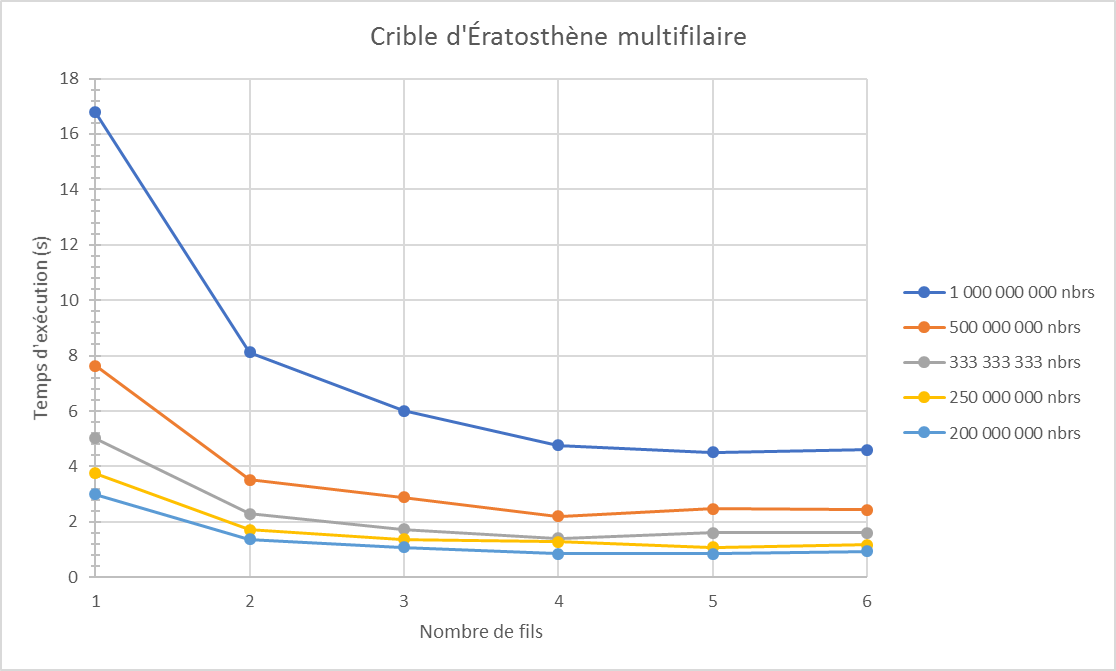
\includegraphics[scale=0.7]{Images/Graph_temps_exec.png}
		\caption{Comparaison des temps d'éxécution}
	\end{figure}
\end{center}

\begin{center}
	\begin{figure}[H]
		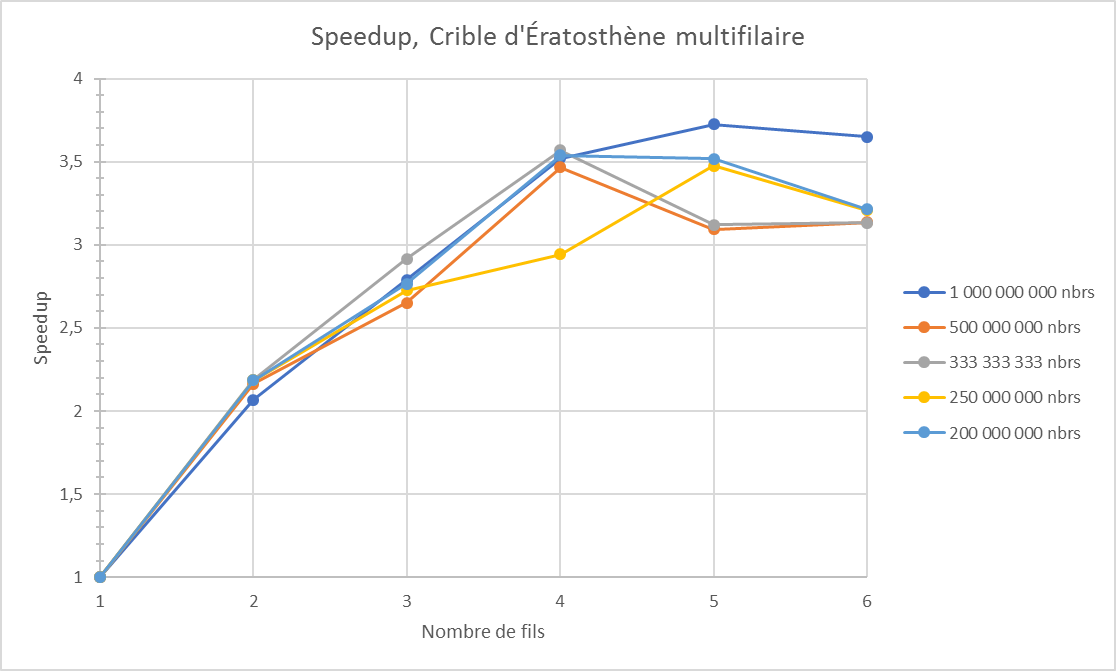
\includegraphics[scale=0.7]{Images/Graph_speedup.png}
		\caption{Comparaison du speedup selon le nombre de fil}
	\end{figure}
\end{center}

\begin{center}
	\begin{figure}[H]
		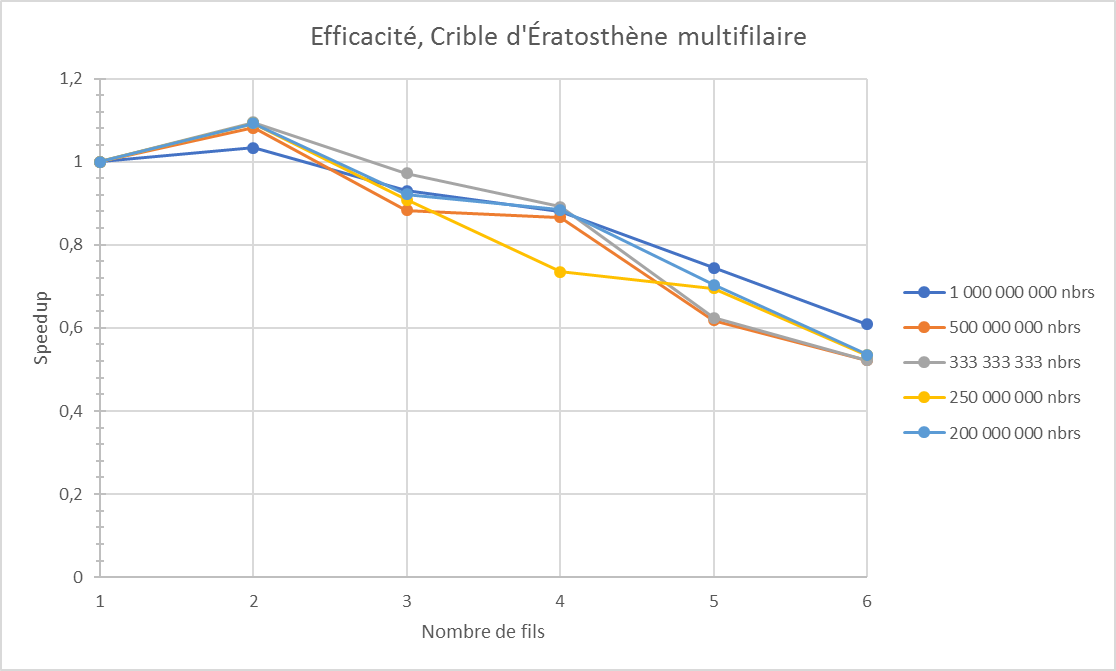
\includegraphics[scale=0.7]{Images/Graph_eff.png}
		\caption{Comparaison de l'éfficacité selon le nombre de fil}
	\end{figure}
\end{center}
\section{Interprétation}

\chapter{Conclusion}

\end{document}
